\section*{Závěr}

Oby dva demodulátory jsem podrobil testu spočívajícího v zašumění vstupního signálu. Hodnoty odstupu signálu od šumu SNR $\in \langle 2; 14 \rangle~dB$. SNR bylo krokováno po $0,05~dB$ a na každou úroveň SNR proběhlo 100~000 demodulačních cyklů.

\begin{figure}[H]
    \centering
    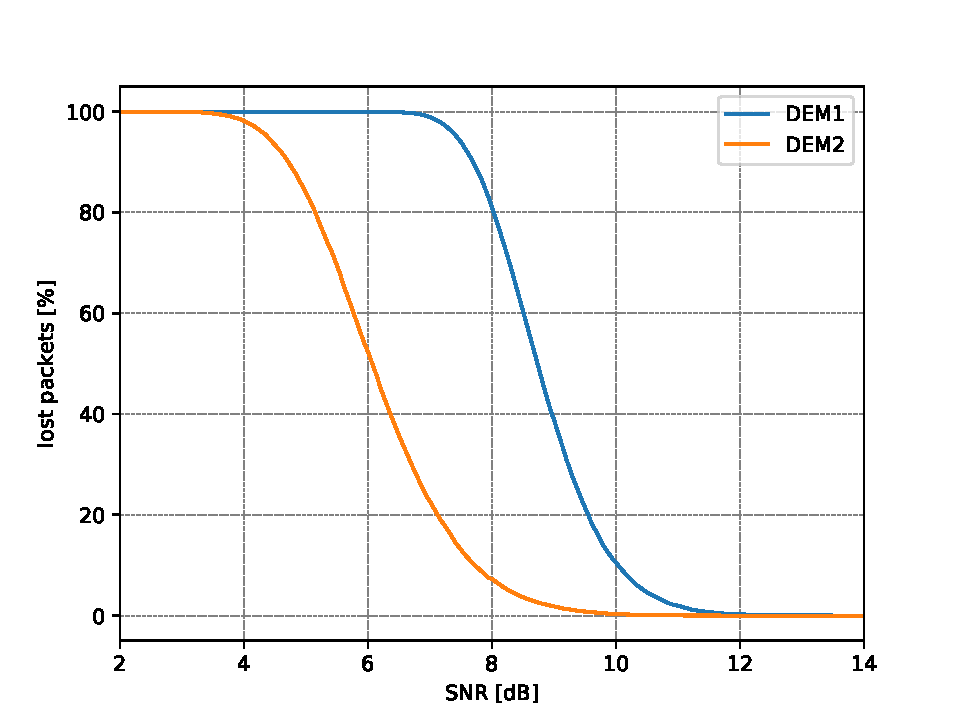
\includegraphics[width=\textwidth]{img/lost_packets.pdf}
    \caption{Závislost chybovosti na SNR}
\end{figure}


\begin{enumerate}
    \item  Z provedeného experimentu lze pozorovat, že DEM1 dosáhne nulové chybovosti při SNR$ = 12~dB$ a DEM2 při SNR$ = 10~dB$. DEM2 je tedy schopen  demodulovat více zašumělý signál.
    \item DEM1 je velmi citlivý na hodnotu prahu, nejlepších výsledků jsem dosáhl s prahem 0,7.
    \item Dalším parametrem který má velký vliv na obě metody demodulátoru jsou filtry. Čím mají filtry větší rozdíl útlumu mezi propustným a nepropustným pásmem tím jsou vhodnější. Také je důležité správně zvolit mezní frekvence filtrů.
\end{enumerate}

\begin{figure}[H]
    \centering
    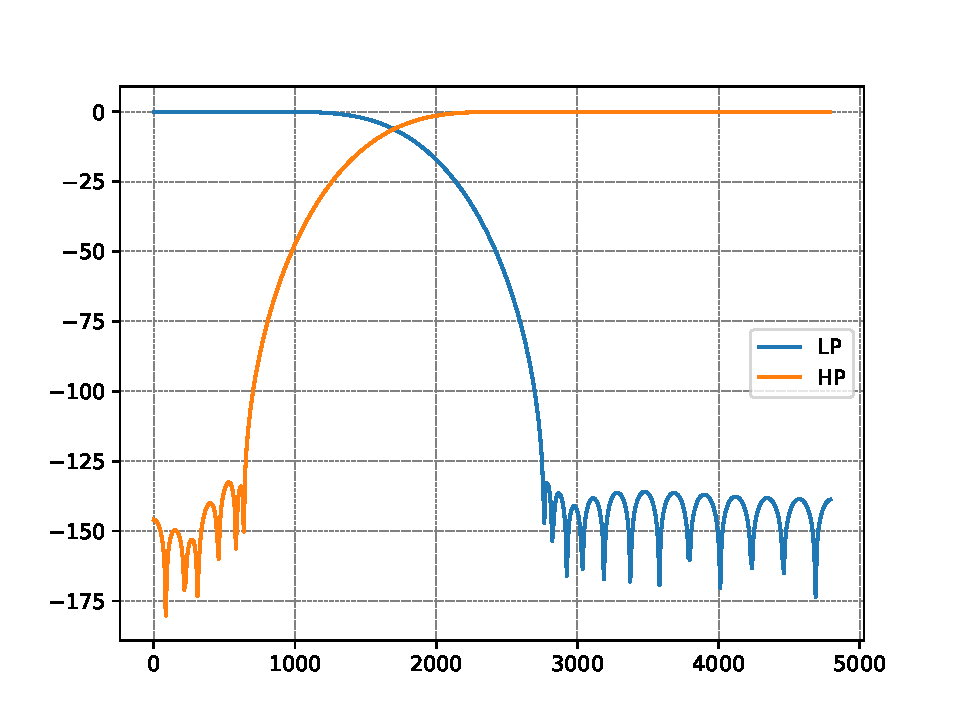
\includegraphics[width=0.8\textwidth]{img/filter.pdf}
    \caption{Frekvenční charakteristiky navržených filtrů}
\end{figure}

Jedná se o FIR filtry, tedy filtry s konečnou impulzní odezvou. Navrženy jsou pomocí metody okna realizované funkcí \texttt{scipy.signal.firwin}, která vrací impulzní odezvu. Délka impulzní odezvy je 41 vzorků. Použité okno je Kaiserovo s parametrem $\beta = 14$.

\begin{lstlisting}[caption={Dekódování zprávy ze souboru \texttt{1.wav}}]
    80 21 01 08 31 30 31 34 | .!..1014
    31 34 34 31 02 04 36 35 | 1441..65
    39 31 07 0F 6C 61 62 2E | 91..lab.
    6D 69 6B 72 6F 70 72 6F | mikropro
    63 65 73 CA F6 FF E6    | ces....

    Packet length 36 octets
    P1 datetime(MM/DD HH:MM): 10/14 14:41
    P2 caller number: 6591
    P7 caller name: lab.mikroproces
\end{lstlisting}

\begin{lstlisting}[caption={Dekódování zprávy ze souboru \texttt{3.wav}}]
    80 1D 01 08 31 30 31 34 | ....1014
    31 34 35 30 02 04 36 35 | 1450..65
    39 35 07 0B 6C 61 62 2E | 95..lab.
    50 43 36 2E 36 30 61 BE | PC6.60a.
    BD DD                   | ..

    Packet length 32 octets
    P1 datetime(MM/DD HH:MM): 10/14 14:50
    P2 caller number: 6595
    P7 caller name:
                    lab.PC6.60a
\end{lstlisting}

Celý demodulátor je napsaný v Pythonu a dostupný na \url{https://github.com/wykys/MIKS-FSK}. Navíc simulace využívá paralelizaci výpočtů na více jader, takže výpočet probíhá relativně rychle.